\chapter{Trigonometria}

\section{Razões Trigonométricas no Triângulo Retângulo}

\subsection{Triângulo Retângulo}


Um Triângulo é dito retângulo quando um de seus ângulos internos é reto. 


\begin{figure}[H]
	\centering
	
	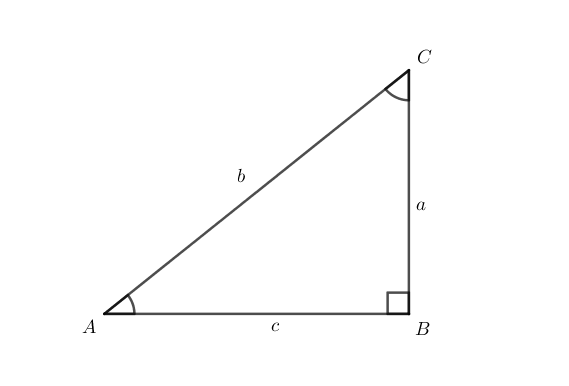
\includegraphics[scale=3.5]{imagens/triangulo-retangulo.png}

\end{figure}

\subsection{Teorema de Pitágoras}
\newtheorem{teorema}{Teorema}
\begin{teorema}
	O quadrado da Hipotenusa é igual à soma do quadrado dos catetos.
\end{teorema}

		$$a^{2}=b^{2}+c^{2}$$ 
		
\newtheorem{proof}{Demonstração}
\begin{proof}
    Vamos demonstrar o teorema de Pitágoras.
\end{proof}

Considere o quadrado de lado $ a $ inscrito no quadrado de lado $ b+c $.

\begin{figure}[H]
	\centering
	
	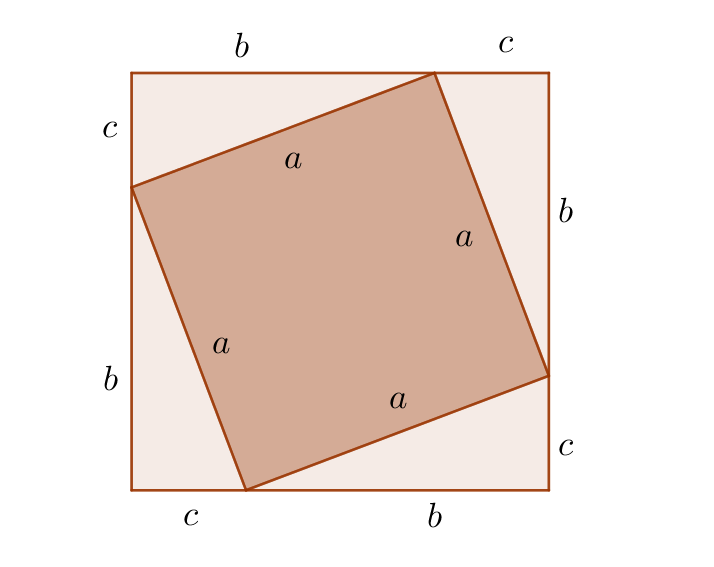
\includegraphics[scale=3.5]{imagens/pitagoras.png}

\end{figure}

A partir da figura acima percebe-se que a área do quadrado $a$ é igual a área do quadrado $b+c$ menos a área dos 4 triângulos de lados $b$ e $c$. Escrevendo essa relação, temos:
$$a^{2} = (b+c)^2 - 4\left(\dfrac{bc}{2}\right)$$

$$a^{2} = b^{2} + 2bc + c^{2} - 2bc$$

$$ a^{2} = b^{2}+c^{2}  $$

\textbf{Observação:}
$\left(\frac{bc}{2}\right)$ é a área do triângulo retângulo de catetos $b$ e $c$.

\subsection{Seno, Cosseno e Tangente}

Considere o triângulo retângulo abaixo:

\begin{figure}[H]
	\centering
	
	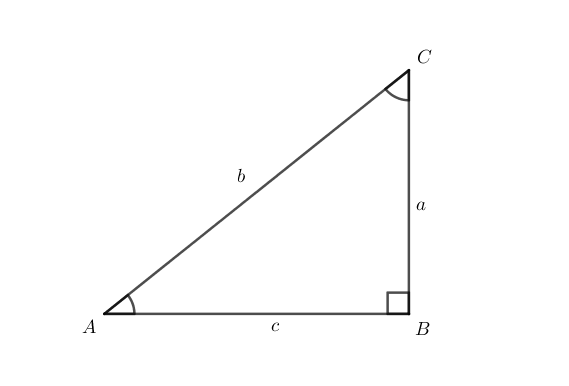
\includegraphics[scale=3.5]{imagens/triangulo-retangulo.png}

\end{figure}

\subsubsection{Seno}
O seno de um ângulo agudo é a razão entre o cateto oposto a esse ângulo e a hipotenusa
$$\sen\hat{A} = \dfrac{a}{b}$$

\subsubsection{Cosseno}
O cosseno de um ângulo agudo é a razão entre o cateto adjacente a esse ângulo e a hipotenusa
$$\cos \hat{A} = \dfrac{c}{b}$$

\subsubsection{Tangente}
A tangente de um ângulo agudo é a razão entre o cateto oposto a esse ângulo e o cateto adjacente.
$$\tg \hat{A} = \dfrac{a}{c}$$

\subsection{Relação Fundamental da Trigonometria}

considere o seguinte triângulo retângulo:

\begin{figure}[H]
	\centering
	
	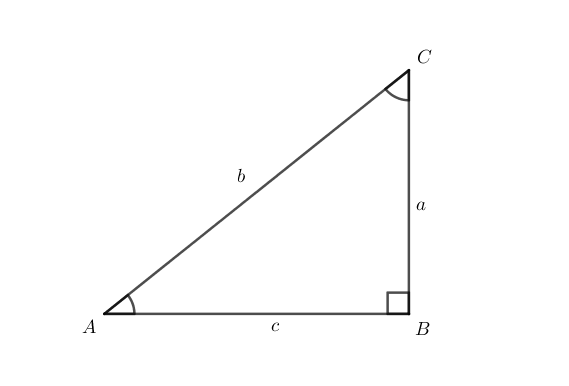
\includegraphics[scale=3.5]{imagens/triangulo-retangulo.png}

\end{figure}

\newtheorem{proof}{Demonstração}
\begin{proof}
Vamos demonstrar a relação fundamental da Trigonometria.
\end{proof}

$$\sen\hat{A} = \dfrac{a}{b} \, \Rightarrow a = b \sen\hat{A} $$


$$\cos \hat{A} = \dfrac{c}{b} \, \Rightarrow c = b \cos \hat{A}$$

Pelo teorema de Pitágoras, temos $ b^{2}=a^{2}+c^{2}$. Substituindo os valores:
$$ b^{2}=( b \sen\hat{A} )^{2}+(b \cos \hat{A})^{2}$$
$$b^{2}= b^{2} \sen^{2}\hat{A} +b^{2} \cos^{2} \hat{A}$$
Dividindo de ambos os lados da equação por $ b^{2}$ temos:

$$\sen^{2}\hat{A} + \cos^{2} \hat{A} = 1 $$

\subsection{Ângulos Complementares}


considere o Triângulo retângulo abaixo:

\begin{figure}[H]
	\centering
	
	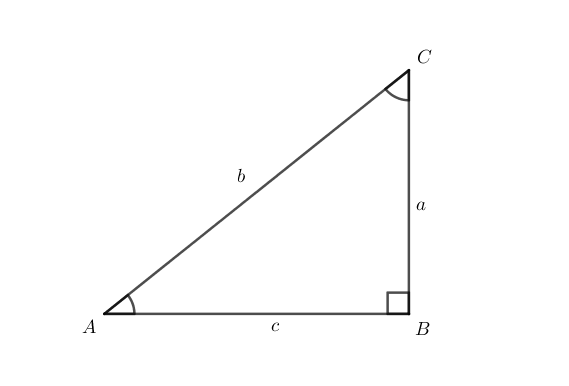
\includegraphics[scale=3.5]{imagens/triangulo-retangulo.png}

\end{figure}


$$
\begin{cases}
\hat{A}+\hat{B}+\hat{C}=180̣^{\circ}
\hat{B} = 90^{\circ}\\
\hat{A} + \hat{C} = 90^{\circ}
\end{cases}
$$

Dizemos que $\hat{A} $ e $ \hat{C} $ são complementares, pois a soma dos dois é igual à $90^{\circ}$. Com isso decorre as seguintes relações:

$$\sen\hat{A} = \dfrac{a}{b}$$

$$\cos\hat{C} = \dfrac{a}{b}$$
\centering
\xymatrix{
*+[F-:<3pt>]{
\sen\hat{A} = \cos\hat{C}}
\\
\\}



$$\cos\hat{A} = \dfrac{c}{b}$$
$$\sen\hat{C} = \dfrac{c}{b}$$
\centering
\xymatrix{
*+[F-:<3pt>]{
\cos\hat{A} = \sen\hat{C} }
\\}

\newpage









%\begin{figure}[H]
%	\centering
%	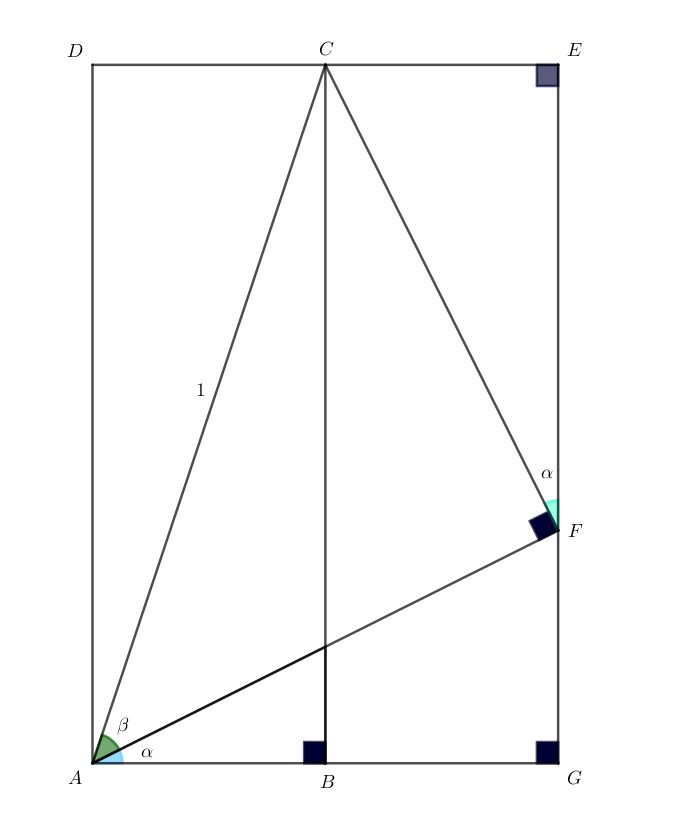
\includegraphics[scale=3.5]{imagens/soma-seno-cosseno.png}
%\end{figure}